\chapter{Nuestra propuesta}
\label{sec:algoritmo}
\section{Agregando probabilidades a un algoritmo existente}

En esta secci\'on se presenta una modificaci\'on del algoritmo
de~\cite{arec2:2008:Areces} donde el orden fijo de las propiedades de
la escena de entrada se sustituye por una distribuci\'on de probabilidad finita. \\

%Los cambios requeridos son bastante sencillos (v\'ease
%Figuras~\ref{algo:bisim-l} y~\ref{algo:bisim-add-el-over}), pero el comportamiento del algoritmo 
%resultante cambia notablemente. 

Con los cambios propuestos el nuevo algoritmo tiene 3 caracter\'isticas nuevas:
\begin{itemize}
 \item Es no determin\'istico: dos ejecusiones del algoritmo con la
misma entrada podr\'{i}an resultar en diferentes REs para los objetos en la escena.\\

 \item Conseguimos mayor sobreespecificaci\'on: simulando lo que encontramos en el corpus.\\

 \item Podemos generar una distribuci\'on de probabilidad
para las ER generadas por el algoritmo si lo ejecutamos muchas veces con
el mismo input. Como vamos a mostrar emp\'{i}ricamente en
Secci\'on~\ref{sec:evaluacion}, dado un corpus de ER para una escena determinada,
es posible calcular una distribuci\'on de probabilidad adecuada para la
probabilidad de uso de las propiedades y relaciones en la escena, de tal manera que
la distribuci\'on de probabilidad de las REs generadas por el modelo
simule la que se encuentra en el corpus.\\
\end{itemize}

Vamos a codificar a las propiedades unarias como relaciones binarias con un
elemento adicional `dummy' en el modelo (por ejemplo, que codifica el hecho de que
$e_1$ es \emph{azul} diciendo que est\'a relacionado con ese elemento ficticio por
la relaci\'on binaria \emph{azul}).
\textcolor{blue}{deberia cambiar el modelo, para mostrar ese elemento dummy del cual se habla, o sacar esa parte, me parece que se entiende mejor sin eso...}

Usaremos la siguiente imagen \ref{GRE3D7-stimulus} como ejemplo para mostrar los pasos a seguir para la ejecuci\'on del algoritmo.

Como los algoritmos nombrados anteriormente, nuestro algoritmo toma como input un modelo de la imagen considerada (un XML con cierta informaci\'on de la imagen), que a modo pr\'actico para que sea visualizable vamos a graficar, como se muestra en la Figura  \ref{GRE3D7-stimulus-graph}. 

\begin{figure}[ht]
\begin{minipage}[b]{0.45\linewidth}
\centering
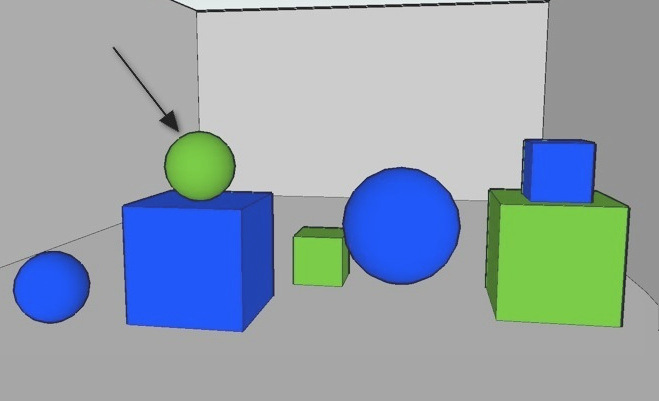
\includegraphics[width=\textwidth]{images/3.jpg}
\vspace*{1cm}
\caption{Escena del GRE3D7}
\label{GRE3D7-stimulus}
\end{minipage}
\hspace*{-0.35cm}
\begin{minipage}[b]{0.6\linewidth}
\centering
\begin{tikzpicture}
  [
    n/.style={circle,fill,draw,inner sep=3pt,node distance=1.4cm},
    aArrow/.style={->, >=stealth, semithick, shorten <= 2pt, shorten >= 2pt},
  ]
 \node[n,label=above:$e_1$,label=below:{
    \relsize{-1}$\begin{array}{c}
      \nLeft\\[-2pt]
      \nSmall\\[-2pt] 
      \nBlue \\[-2pt] 
      \nBall\end{array}$}] (a) {};

 \node[n,label=above:$e_2$,label=below:{
    \relsize{-1}$\begin{array}{c}
      \nLeft\\[-2pt]
      \nBig\\[-2pt] 
      \nBlue\\[-2pt] 
      \nCube\end{array}$}, right of=a] (b) {};

 \node[n,label=below:$e_3$,label=above:{
    \relsize{-1}$\begin{array}{c}
      \nTop\\[-2pt]
      \nLeft\\[-2pt]
      \nSmall\\[-2pt] 
      \nGreen\\[-2pt] 
      \nBall\end{array}$}, above of=b] (c) {};

 \node[n,label=above:$e_4$,label=below:{
    \relsize{-1}$\begin{array}{c}
      \nSmall\\[-2pt] 
      \nGreen\\[-2pt] 
      \nCube\end{array}$}, right of=b] (d) {};

 \node[n,label=above:$e_5$,label=below:{
    \relsize{-1}$\begin{array}{c}
      \nBig\\[-2pt] 
      \nBlue\\[-2pt] 
      \nBall\end{array}$}, right of=d] (e) {};

 \node[n,label=above:$e_6$,label=below:{
    \relsize{-1}$\begin{array}{c}
      \nBig\\[-2pt] 
      \nGreen\\[-2pt] 
      \nCube\end{array}$}, right of=e] (f) {};

 \node[n,label=below:$e_7$,label=above:{
    \relsize{-1}$\begin{array}{c}
      \nTop\\[-2pt]
      \nSmall\\[-2pt] 
      \nBlue\\[-2pt] 
      \nCube\end{array}$}, above of=f] (g) {};

 \draw [aArrow,bend right=90] (b) to node[auto,swap]{\relsize{-1}$\nBelow$} (c);
 \draw [aArrow,bend right=90] (c) to node[auto,swap]{\relsize{-1}$\nOntop$} (b);

 \draw [aArrow,bend right=30] (d) to node[auto,swap]{\relsize{-1}$\nLeftof$} (e);
 \draw [aArrow,bend right=30] (e) to node[auto,swap]{\relsize{-1}$\nRightof$} (d);

 \draw [aArrow,bend right=90] (f) to node[auto,swap]{\relsize{-1}$\nBelow$} (g);
 \draw [aArrow,bend right=90] (g) to node[auto,swap]{\relsize{-1}$\nOntop$} (f);

 \draw[dotted] (-.5,-1.4) rectangle (7.1,3.1);

 \end{tikzpicture}
\caption{Escena como un modelo relacional}
\label{GRE3D7-stimulus-graph}
\end{minipage}
\end{figure}

%It is clear that a scene can be encoded in different ways as a relational model (for example, we could argue that $e_1$ is also \emph{leftof} $e_2$, and so on).  The algorithm assumes that these issues have been resolved and that the model encodes a suitable representation of the scene we want to describe.  Moreover, we will assume that all relations are \emph{binary}.  We will not consider relations of arity greater than two (relations of higher arity can be encoded as binary relations via reification, if necessary), and unary
%properties can be encoded as binary relations including one additional `dummy' element in the model (e.g., we encode the fact that $e_1$ is \emph{blue} saying that it is related to the dummy element by the \emph{blue} binary relation).

%On termination, the algorithm computes what are called the $\mathcal{L}$-similarity classes of the input model $\gM$. Intuitively, if two elements in the model belong to the same $\mathcal{L}$-similarity class, then $\mathcal{L}$ is not expressive enough to tell them appart (i.e, no formula in $\mathcal{L}$ can distinguish them). 

%In what follows, we will use formulas of the $\el$ description logic language~\cite{baad:desc03} to describe refinement classes.  As discussed in~\cite{arec2:2008:Areces}, this language is suitable for conjunctive relational RE, which are the ones we will find in the corpora used for our evaluation\footnote{Notice, though, that the particular formal language used is independent of the main algorithm, and different add$_{\mathcal{L}}$(R,$\varphi$,\RE) functions can be used depending on the language involved.}. For a detail description of $\el$, we refer to~\cite{baad:desc03}.  For this paper, we only need to know that the interpretation of the formula $\psi \sqcap \exists$R.$\varphi$ is the set of all elements that satisfy $\psi$ and that are related by relation R to some element that satisfy $\varphi$. For example, the interpretation of the formula \emph{ball} $\sqcap \exists$\emph{leftof}.\emph{cube} is the set of all balls that are on the left of some cube.  

%We are now ready to describe Algorithms~\ref{algo:bisim-l}
%and~\ref{algo:bisim-add-el}. Algorithm~\ref{algo:bisim-l} takes as
%input a model $\gM$ and a list Rs of pairs (R,R.\puse) that links each
%relation R to some probability of use R.\puse. I.e., if $\REL$ is the
%set of all relation symbols in the model (i.e., the \emph{signature}
%of the model) then Rs $\in (\REL \times [0,1])^*$. Moreover, we assume
%Rs to be ordered by R.\puse.

\begin{figure}[!t]
\small
\centering
\begin{algorithm}[H]
\dontprintsemicolon
\caption{Computing $\mathcal{L}$-similarity classes}\label{algo:bisim-l}
\KwIn{\footnotesize A model $\gM$ and a list Rs $\in (\REL \times [0,1])^*$
 of relation symbols with their \puse\ values, ordered by \puse}
\KwOut{\footnotesize A set of formulas \RE such that
$\{\interp{\varphi} \mid \varphi \in \RE\}$ is the set of
$\mathcal{L}$-similarity classes of $\gM$}

$\RE \leftarrow \{\top\}$\tcp*[f]{\footnotesize the most general description $\top$ applies to all elements in the scene}

\For{\em (R,R.\puse) $\in$ Rs}{
	R.\randomuse = Random(0,1)\tcp*[f]{\footnotesize R.\randomuse is the probability of using R} \;
        R.\incuse = (1 $-$ R.\puse) / MaxIterations\tcp*[f]{\footnotesize R.\puse\ are incremented by R.\incuse in each loop}
}

\Repeat{\em $\forall$((R,R.\puse) $\in$ Rs).(R.\puse $\ge$ 1)\tcp*[f]{\footnotesize R.\puse\ are incremented until they reach 1}}{
  \While(\tcp*[f]{\footnotesize while some class has at least two elements}){\em $\exists (\varphi \in$ \RE)$.(\#\interp{\varphi}>1)$}{
      \RE' $\leftarrow$ \RE \tcp*[f]{\footnotesize make a copy for future comparison} \;
      \For{\em (R, R.\puse) $\in$ Rs}{
          \If(\tcp*[f]{\footnotesize R will be used in the expression}){\em R.\randomuse $\le$ R.\puse}{
              \lFor{\em $\varphi \in$ \RE}{
                  add$_\mathcal{EL}$(R, $\varphi$, \RE)\tcp*[f]{\footnotesize refine all classes using R}}
                  }\;
              \If(\tcp*[f]{\footnotesize the classification has changed}){\em \RE $\not =$ \RE'}{exit\tcp*[f]{\footnotesize exit for-loop to try again highest R.\puse}}
              }
     \If(\tcp*[f]{\footnotesize the classification has stabilized}){\em \RE $=$ \RE'}{exit\tcp*[f]{\footnotesize exit while-loop to increase R.\puse}}
  }
  \lFor{\em (R,R.\puse) $\in$ Rs}{
    R.\puse $\leftarrow$ R.\puse $+$ R.\incuse\tcp*[f]{\footnotesize increase R.\puse}
  }
}
\end{algorithm}

\begin{algorithm}[H]
\dontprintsemicolon
\caption{add$_\el$(R, $\varphi$, \RE)} \label{algo:bisim-add-el-over}

\If(\tcp*[f]{\footnotesize are we in the first loop?}){\em FirstLoop?}{
    Informative $\leftarrow$ TRUE \tcp*[f]{\footnotesize allow overspecification}}
\lElse(\tcp*[f]{\footnotesize informative: smaller than the original?}) {Informative $\leftarrow$ $\interp{\psi \sqcap \exists \mbox{\em R}.\varphi} \neq \interp{\psi}$} 
\For{\em $\psi \in$ \RE with $\#\interp{\psi} > 1$}{
  \If{\em $\psi \sqcap \exists$R.$\varphi$ is not subsumed in \RE\ {\bf and} \tcp*[f]{\footnotesize non-redundant: can't be obtained from \RE?}\\
    \em \ \ \ $\interp{\psi \sqcap \exists \mbox{\em R}.\varphi} \neq \emptyset$ {\bf and} \tcp*[f]{\footnotesize non-trivial: has elements?}\\
     \ \ \  \emph{Informative}}{
    add $\psi \sqcap \exists \mbox{R}.\varphi$ to $\RE$ \tcp*[f]{\footnotesize add the new class to the classification} \;
    remove subsumed formulas from $\RE$ \tcp*[f]{\footnotesize remove redundant classes}
  }
}
\end{algorithm}
\vspace*{-.5cm}\caption{Algoritmos de refinamiento con probabilidades y sobrespecificacion para el \el-language}\label{fig:algo3}

\end{figure}


Ahora estamos listos para describir los algoritmos~\ref{algo:bisim-l}
y~\ref{algo:bisim-add-el-over}. El algoritmo~\ref{algo:bisim-l} toma como
entrada un modelo $\gM$ y una lista de pares de tuplas (R, R.\puse) que vinculan a cada
relaci\'on R a una cierta probabilidad de uso R.\puse. Es decir, si $\REL$ es el
conjunto de todos los s\'imbolos de relaci\'on en el modelo (es decir, la~\emph{signatura}
del modelo), recordemos que tomamos las unarias como relaciones, entonces R $\in (\REL \times [0,1])^*$. Por otra parte, asumimos que R esta ordenada por R.\puse\ de mayor a menor.
\textcolor{blue}{deberia reemplazar aca que R es un conjunto por una lista ordenada...}

%\begin{figure}[t]
%\small
%\centering
%\begin{algorithm}[H]
%\dontprintsemicolon
%\caption{Computing $\mathcal{L}$-similarity classes}\label{algo:bisim-l}
%\KwIn{\footnotesize A model $\gM$ and a list Rs $\in (\REL \times [0,1])^*$
 %of relation symbols with their \puse\ values, ordered by \puse}
%\KwOut{\footnotesize A set of formulas \RE such that
%$\{\interp{\varphi} \mid \varphi \in \RE\}$ is the set of
%$\mathcal{L}$-similarity classes of $\gM$}
%
%$\RE \leftarrow \{\top\}$\tcp*[f]{\footnotesize the most general description $\top$ applies to all elements in the scene}
%
%\For{\em (R,R.\puse) $\in$ Rs}{
	%R.\randomuse = Random(0,1)\tcp*[f]{\footnotesize R.\randomuse is the probability of using R} \;
        %R.\incuse = (1 $-$ R.\puse) / MaxIterations\tcp*[f]{\footnotesize R.\puse\ are incremented by R.\incuse in each loop}
%}
%
%\Repeat{\em $\forall$((R,R.\puse) $\in$ Rs).(R.\puse $\ge$ 1)\tcp*[f]{\footnotesize R.\puse\ are incremented until they reach 1}}{
  %\While(\tcp*[f]{\footnotesize while some class has at least two elements}){\em $\exists (\varphi \in$ \RE)$.(|\interp{\varphi}|>1)$}{
      %\RE' $\leftarrow$ \RE \tcp*[f]{\footnotesize make a copy for future comparison} \;
      %\For{\em (R, R.\puse) $\in$ Rs}{
          %\If(\tcp*[f]{\footnotesize R will be used in the expression}){\em R.\randomuse $\le$ R.\puse}{
              %\For{\em $\varphi \in$ \RE}{
                  %add$_\mathcal{L}$(R, $\varphi$, \RE)\tcp*[f]{\footnotesize refine all classes using R}}
                  %}\;
              %\If(\tcp*[f]{\footnotesize the classification has changed}){\em \RE $\not =$ \RE'}{exit\tcp*[f]{\footnotesize exit for-loop to try again highest R.\puse}}
              %}
     %\If(\tcp*[f]{\footnotesize the classification has stabilized}){\em \RE $=$ \RE'}{exit\tcp*[f]{\footnotesize exit while-loop to increase R.\puse}}
  %}
  %\For{\em (R,R.\puse) $\in$ Rs}{
    %R.\puse $\leftarrow$ R.\puse $+$ R.\incuse\tcp*[f]{\footnotesize increase R.\puse}
  %}
%}
%\end{algorithm}
%\vspace*{-.5cm}\caption{Main algorithm, dealing with probabilities}\label{fig:algo1}
%\end{figure}
%
%
%\begin{figure}[t]
%\small
%\centering
%\begin{algorithm}[H]
%\dontprintsemicolon
%\caption{add$_\el$(R, $\varphi$, \RE)} \label{algo:bisim-add-el}
%
%\For{\em $\psi \in$ \RE with $|\interp{\psi}| > 1$}{
  %\If(\tcp*[f]{\footnotesize informative:smaller than the original?}){\em $\psi \sqcap \exists$R.$\varphi$ is not subsumed in \RE\ {\bf and} \tcp*[f]{\footnotesize non-redundant:can't be obtained from \RE?}\\
    %\em \ \ \ $\interp{\psi \sqcap \exists \mbox{\em R}.\varphi} \neq \emptyset$ {\bf and} \tcp*[f]{\footnotesize non-trivial:has elements?}\\
     %\ \ \ $\interp{\psi \sqcap \exists \mbox{\em R}.\varphi} \neq \interp{\psi}$ }{
    %add $\psi \sqcap \exists \mbox{R}.\varphi$ to $\RE$ \tcp*[f]{\footnotesize add the new class to the classification} \;
    %remove subsumed formulas from $\RE$ \tcp*[f]{\footnotesize remove redundant classes}
  %}
%}
%\end{algorithm}
%\vspace*{-.5cm}\caption{Refinement function for the \el-language}\label{fig:algo2}
%\end{figure}

%The set $\RE$ will contain the formal description of the refinement
%classes and it is initialized by the most general description $\top$.
%For each R, we first compute R.\randomuse, a random number in [0,1].
%If R.\randomuse $\le$ R.\puse\ then we will use R to refine the set of
%classes.  The value of R.\puse\ will be incremented by $R.\incuse$ in
%each main loop, to ensure that all relations are, at some point,
%considered by the algorithm.  This ensures that a referring expression
%will be found if it exist; but gives higher probability to expressions
%using relations with a high R.\puse.
% 
%While $\RE$ contains descriptions that can be refined (i.e., classes
%with at least two elements) we will call the refinement function
%add$_\mathcal{L}$(R,$\varphi$,$\RE$) successively with each relation
%in Rs. A change in one of the classes, can trigger changes in
%others. For that reason, if $\RE$ changes, we exit the for-loop to
%start again with the relations of higher R.\puse. If the after trying
%to refine the set with all relations in Rs, the set $\RE$ has not
%changed, the we have reach a stable state (i.e., the classes described
%in $\RE$ cannot be further refined, using the current R.\puse\
%values). We will then increment all the R.\puse\ values and start the
%procedure again.

%Algorithm~\ref{algo:bisim-add-el} coincides with the one described
%in~\cite{arec2:2008:Areces}.  It will refine each of the descriptions
%in $\RE$ using the relation R and the other descriptions already in
%$\RE$, under certain conditions. The new description should be
%\emph{non-redundant} (the new class cannot be obtained as the union of
%classes already represented in $\RE$), \emph{non-trivial} (the new
%class is not empty), and \emph{informative} (the new class should not
%coincide with the original class).  If all this conditions are met,
%the new description is added to $\RE$, and redundant descriptions
%possible created by the addition of the new description are
%eliminated.

%Suppose fixed an input model $\gM$ and values for Rs, and fix also
%some target element $t$.  Assume also that $t$ indeed has an
%$\el$-referring expression.  Upon termination,
%Algorithm~\ref{fig:algo1} will compute an $\el$ formula $\varphi$ such
%that $\interp{\varphi} = \{t\}$, but $\varphi$ might be different in
%each run of the algorithm (even though $\gM$ and Rs are fixed).  If we
%repeat this experiment a statistically significant number of times, we
%can define an estimate of the probability distribution of the REs
%generated by the algorithm for $t$, given $\gM$ and Rs. In
%Section~\ref{sec:evaluation} we will show that given a corpus of REs
%for $\gM$, it is possible to define R.\puse\ values so that this
%probability distribution matches with good accuracy the probability
%distribution of REs found in the corpus.


El conjunto $\RE$ contendr\'a la descripci\'on formal de las clases de refinamiento
y es inicializado por la descripci\'on m\'as general $\top$.
Para cada R, primero calculamos R.\randomuse, un n\'umero aleatorio en [0,1].
Si R.\randomuse $\le$ R.\puse\ entonces vamos a utilizar R para refinar el conjunto de
clases. El valor de R.\puse\ se incrementar\'a en $R.\incuse$
en cada ciclo principal, para asegurar que todas las relaciones son en alg\'un momento,
consideradas por el algoritmo. Esto asegura que una expresi\'on referencial
se encontrar\'a si existe; pero dar\'a mayor probabilidad a las expresiones
que usan las relaciones con m\'as alta R.\puse.
 
Mientras que $\RE$ contiene descripciones que pueden ser refinadas (es decir, clases
con al menos dos elementos) vamos a llamar a la funci\'on de refinamiento
add$_\mathcal{L}$(R,$\varphi$,$\RE$) sucesivamente con cada relaci\'on
de Rs. Un cambio en una de las clases, puede desencadenar cambios en
las otras. Por esa raz\'on, si $\RE$ cambia, salimos del ciclo for y volvemos a
empezar con las relaciones de m\'as alta R.\puse. Si despu\'es de probar refinar el conjunto con todas las relaciones de Rs, el conjunto $\RE$ no ha
cambiado, hemos alcanzado un estado estable (es decir, las clases que se describen
en $\RE$ no puede ser refinadas, utilizando los valores de R.\puse\ ). 
A continuaci\'on, se incrementar\'an todos los valores de R.\puse\ y se iniciar\'a el
procedimiento de nuevo.

El algoritmo~\ref{algo:bisim-add-el} coincide con el descripto
en~\cite{arec2:2008:Areces}. Se refinar\'a cada una de las descripciones
en $\RE$ utilizando la relaci\'on R y las otras descripciones que ya est\'an en
$\RE$, bajo ciertas condiciones. La nueva descripci\'on debe ser
\emph{no redundante} (la nueva clase no se puede obtener como la uni\'on de
clases ya representadas en $\RE$), \emph{no trivial} (la nueva
clase no es vac\'{i}a), es \emph{informativa} (la nueva clase no debe
coincidir con la clase original). Si se cumplen todas estas condiciones,
la nueva descripci\'on se a\~nade a $\RE$, y las descripciones redundantes
posiblemente creadas por la adici\'on de la nueva descripci\'on son
eliminadas.

Supongamos que se fija un modelo de entrada $\gM$ y los valores de R.\puse, y se fija tambi\'en
alg\'un elemento target $t$. Supongamos tambi\'en que $t$ tiene una expresi\'on referencial en 
$\el$. Cuando termine el
Algoritmo~\ref{fig:algo1} habr\'a calculado una f\'ormula $\varphi$ de $\el$ tal
que $\interp{\varphi} = \{t\}$, pero $\varphi$ pueden ser diferentes en
cada ejecuci\'on del algoritmo (a pesar de que $\gM$ y Rs son fijos). Si nosotros
repetimos este procedimiento un n\'umero estad\'{i}sticamente significativo de veces,
podemos definir una estimaci\'on de la distribuci\'on de probabilidad de las ER
generadas por el algoritmo para $t$, dado $\gM$ y Rs. En la
Secci\'on~\ref{sec:evaluacion} vamos a demostrar que dado un corpus de ER
para $\gM$, es posible definir los valores de R.\puse\ para que esta
distribuci\'on de probabilidad coincida con buena precisi\'on a la distribuci\'on de probabilidad
 de ER que se encuentra en el corpus.






\subsection{Aprendizaje autom\'atico desde un corpus para describir nuevos objetos}
\label{sec:learning}

%In the previous section we presented an algorithm that assumes that
%each relation R used in a referring expressions has a known
%probability of use R.\puse. In this section, we describe how to
%calculate these probabilities from corpora.  The general set up is the
%following:we assume available a corpus of REs associated to different
%scenes that are typical of the domain in which the GRE algorithm will
%have to operate.  We show first how to calculate R.\puse\ values for
%those scenes for which a corpus of REs is available.  We then show how
%to generalize these values to other scenes in the domain, using a
%machine learning algorithm. \textit{First we} will exemplify the
%methodology using the GRE3D7 corpus which we introduce in the Section
%~\ref{sec:learningGRE} and then we will show how to do the same with
%the TUNA-corpus that we describe in Section~\ref{sec:learningTUNA}.


En la secci\'on anterior hemos presentado un algoritmo que supone que para
cada relaci\'on R se tiene una conocida
probabilidad de uso R.\puse. En esta secci\'on, se describe c\'omo
calcular estas probabilidades a partir de corpus. Asumimos disponible un corpus de ER asociada a diferentes
escenas t\'{i}picas del dominio en el que el algoritmo GRE tiene que operar. Mostramos primero c\'omo calcular los valores de R.\puse\ para
esas escenas para las que se dispone de un corpus de ER. A continuaci\'on, mostramos c\'omo
generalizar estos valores a otras escenas en el dominio, utilizando un
algoritmo de aprendizaje autom\'atico. En primer lugar vamos a ejemplificar la
metodolog\'{i}a utilizando el corpus GRE3D7 que introducimos en ~\ref{sec:corpusGRE} y, a continuaci\'on mostraremos c\'omo hacer lo mismo con el corpus TUNA introducido en~\ref{sec:corpusTUNA}.


\subsubsection{Calculando \puse\ cuando hay disponible un corpus para la escena considerada}

%Suppose we want to automatically generate REs for target $t$ in a
%given scene, and that we do have available a corpus $C$ of REs for $t$
%in that scene (this is exactly the kind of information we find in the
%GRE3D7 corpus \textit{and in the TUNA-corpus}).  We use the REs in $C$
%to define the relational model used by the algorithm.  Then we
%estimate the value of \puse\ for each of the relations in the model as
%the percentage of REs in which the relation appears.  I.e.,
%\begin{equation}\label{eq1}
%R.\puse = \frac{\# \mbox{ of REs in $C$ in which R appears}}{\# \mbox{ of REs in $C$}}.
%\end{equation}

%In the case of the TUNA corpus the calculation is not neccesary
%because we have only one RE for each scene.

%This estimation is overly simplified and, for example, it does not
%differentiate between the properties of a target and the properties of
%a landmark object used in a relational RE to complete the description
%of the target.  But it is extremely easy to compute, and we will see
%in Section~\ref{sec:evaluation} that it already produces natural REs
%that match those found in the corpus.

%To clarify the computation of R.\puse\ and the model $\gM$ associated
%to each scene we list the required steps in detail, and discuss how we
%carried them out in the GRE3D7 corpus:

Supongamos que queremos generar autom\'aticamente ER para el target $t$ en una
determinada escena, y que tenemos disponible un corpus $C$ de ER de $t$
en esa escena (esto es exactamente el tipo de informaci\'on que encontramos en el
GRE3D7 corpus \textit{y en el TUNA-corpus}). Utilizamos las ER de $C$
para definir el modelo relacional utilizado por el algoritmo. Entonces 
estimaremos el valor de \puse\ para cada una de las relaciones en el modelo como el
porcentaje en que aparece la relaci\'on en las ER. Es decir,
\begin{equation} \label{eq1}
R.\puse = \frac {\#\mbox{de ERs en $C$ en el que aparece R}} {\#\mbox{de las ER en $C$}}.
\end{equation}

En el caso del corpus TUNA el c\'alculo no es necesario
porque tenemos solo una RE para cada escena.

Esta estimaci\'on es demasiado simplificada y, por ejemplo, no 
diferencia las propiedades del target y las propiedades de
los landmarks utilizadas en una RE relacional para completar la descripci\'on
del target. Pero es muy f\'acil de calcular, y vamos a ver
en la Secci\'on~\ref{sec:evaluacion} que ya produce ER naturales
que coinciden con las encontradas en el corpus.

Para aclarar el c\'alculo de R.\puse \ en el modelo $\gM$ asociado
a cada escena enumeramos los pasos necesarios en detalle, y discutimos c\'omo
ellos son llevados a cabo en el corpus GRE3D7:


\begin{enumerate}
%\item Tokenize the referring expressions and call the set of tokens
%  $T$. In particular, multi-word expressions like ``on top of''
%  should be matched to a single token like \emph{ontop}.

%\item Remove hyperonyms from $T$. E.g., if both \emph{cube} and
%  \emph{thing} appear in $T$, delete \emph{thing}.

%\item If the set of tokens obtained in the previous steps contains
%  synonyms normalize them to a representative in the synonym class,
%  and call the resulting set $\REL$; it will be the signature of the
%  model $\gM$ used by the algorithm. E.g., the tokens \emph{little}
%  and \emph{small} are both represented by the token \emph{small}.

%\item For each scene, define $\gM$ such that the interpretation
%  $\interp{\cdot}$ ensures that all the REs in the corpus are REs in
%  the model.  E.g., the $\el$ formulas corresponding to the REs in
%  Table~\ref{corpus-distribution} should all denote the target in the
%  model $\gM$ depicted in
%  Figure~\ref{GRE3D7-stimulus-graph}.

%\item For each R $\in \REL$ compute R.\puse\ using~(\ref{eq1}) if we
%  ave many RE for each scene or we assign 1 to R.\puse\ if R occurs in
%  the RE, we assign 0 otherwise.

\item Tokenizar las expresiones referenciales y llamar al conjunto de palabras
 $T$. En particular, las expresiones de varias palabras como ``arriba de'', ``encima de''
  debe ser igualado a un \'unica palabra que signifique lo mismo, digamos \emph{ontop}.

\item Eliminar hiper\'onimos de $T$. Por ejemplo, si ambos \emph{cubo} y
  \emph{cosa} aparecen en $T$, eliminar \emph{cosa}.

\item Si el conjunto de palabras obtenidas en los pasos anteriores contiene
  sin\'onimos normalizarlos con un representante de la clase,
  y llamar al conjunto resultante $\REL$; que ser\'a la signatura del
  modelo $\gM$ utilizada por el algoritmo. Por ejemplo, las palabras \emph{chico}
  y \emph{peque\~no} son ambas representadas por la palabra \emph{peque\~no}.

\item Para cada escena, definir $\gM$ tal que la interpretaci\'on
 $\interp {\cdot}$ asegure de que todas las ERs encontradas en el corpus sean ER en
  el modelo. Por ejemplo, las $\el$ f\'ormulas correspondientes a la tabla~\ref{results-algo-fig3} deben denotar el target en el
  modelo $\gM$ representado en
  Figura~\ref{GRE3D7-stimulus}.

\item Para cada R$\in \REL$ c\'alculo R.\puse \ utilizando~(\ref{eq1}) si
  hay muchas RE para cada escena o asignamos 1 a R.\puse \ si R se produce en
  el RE, asignamos 0 en caso contrario.


\end{enumerate}

%Steps 1-5 above are easy to carry out (actually, the tokenization and
%normalization steps were already done in the GRE3D7 corpus).  Starting
%from the scene in Figure~\ref{GRE3D7-stimulus} and the corresponding
%corpus shown in Table~\ref{corpus-distribution}, the resulting
%signature and their associated \puse\ are listed in the first three
%columns of Table~\ref{probability-of-use}.

%Notice that the values R.\puse\ obtained in this way should be
%interpreted as the probability of using R to describe the target in
%model $\gM$, and we could argue that they are correlated to the
%\emph{saliency} of R in the model.  For that reason, for example, the
%value of \emph{ball}.\puse\ is 1, while the value of
%\emph{cube}.\puse\ is 0.178.  These probabilities will not be useful
%to describe different targets in different scenes.  We will see how we
%can use them to obtain values for new targets and scenes using a
%machine learning approach in the next section.  Not surprisingly,
%using these values for R.\puse\ the REs generated most often by the
%algorithm can be found in the corpus.  More interestingly, as we
%discuss in Section~\ref{sec:evaluation} the algorithm generates REs
%with a distribution that matches the one found in the corpus and, as
%Table~\ref{results-algo-fig3} shows, even the generated REs not found
%in the corpus are natural.

Los pasos 1-5 anteriores son f\'aciles de llevar a cabo (en realidad, la tokenizaci\'on y
pasos de normalizaci\'on ya se realizaron en el corpus GRE3D7). 
%no se entiende
Comienzo
de la escena en la Figura~\ref{GRE3D7-stimulus} y el correspondiente
corpus muestra en la tabla~\ref{corpus-distribution}, la signatura resultante
y su asociado \puse\ figuran en las tres primeras
columnas de la tabla~\ref{probability-of-use}.


\begin{table}[h!]
\begin{center}
\begin{tabular}{|l|c|c|}
\hline
Expresiones Referenciales & Cantidad de ocurrencias & Porcentage \\
\hline
green ball & 91 & 65.00\% \\
small green ball & 23 & 16.43\% \\
small green ball on top of large blue cube & 8 & 5.71\% \\
green ball on top of blue cube & 5 & 3.57\% \\
green ball on top of large blue cube & 5 & 3.57\% \\
small green ball on top of blue cube & 2 & 1.43\% \\
ball on top of cube & 1 & 0.71\% \\
small green ball on top of large blue cube to the left & 1 & 0.71\% \\
small ball on top large cube & 1 & 0.71\% \\
green ball on top & 1 & 0.71\% \\
small ball on top of small cube & 1 & 0.71\% \\
green ball on top of cube & 1 & 0.71\% \\
\hline
\end{tabular}
\caption{Expresiones Referenciales producidas por las personas para la Figura~\ref{GRE3D7-stimulus}}\label{corpus-distribution}
\end{center}
\end{table}


Observe que los valores R.\puse\ obtenidos de esta manera debe ser
interpretados como la probabilidad de utilizar R para describir el target en
modelo de $\gM $, y podr\'{i}amos argumentar que se correlacionan con la
 prominencia de R en el modelo. Por esa raz\'on, por ejemplo, el
valor de \emph{pelota}.\puse\ es 1, mientras que el valor de
\emph{cubo}.\puse\ es 0.178. Estas probabilidades no ser\'an \'utiles
para describir los diferentes targets en diferentes escenas. Veremos c\'omo se
pueden utilizarlas para obtener valores para los nuevos targets y escenas utilizando un
enfoque de aprendizaje autom\'atico en la siguiente secci\'on. No es de extra\~nar,
que usando estos valores para R.\puse\ las ER generadas con mayor frecuencia por el
algoritmo se puedan encontrar en el corpus. Como discutiremos en la Secci\'on~\ref{sec:evaluacion} el algoritmo genera ER
con una distribuci\'on que coincide con la encontrada en el corpus y, como la
Tabla~\ref{results-algo-fig3} muestra, incluso las ER generadas por el algoritmo que no se encontraron
en el corpus son naturales.


\subsubsection{Calculando \puse\ para el target para escenas sin corpus } 
\label{subsec:learning}

%If there is no corpora that describes the target we can estimate the
%\puse~from corpora on a different scenes in the same domain.
%
%We use simple features to obtain the function, all the features can be
%extracted automatically from the relational model and are listed in

Si no hay corpus de expresiones referenciales que describen el target, se puede estimar la \puse a partir de corpus en un
diferentes escenas en el mismo dominio.
Usamos caracter\'isticas simples para obtener una funci\'on que nos dar\'a la probabilidad de cada palabra en el nuevo modelo, todas las caracter\'isticas que se pueden extraer de forma autom\'atica desde el modelo relacional y se enumeran en la Tabla~\ref{features}.

\begin{small}
\begin{table}[h]
\begin{center}
\begin{tabular}{|l|p{10cm}|}
\hline
target & cuando el elemento target tiene la propiedad. \\
\#rel-prop & n\'umero de propiedades y relaciones que el target tiene.\\
\#rel & n\'umero de relaciones que el target tiene. \\
landmark & cuando un landmark de el target tiene la propiedad, un objeto es un landmark si tiene una relaci\'on directa en el modelo, con el target (lo usamos para el GRE3D7).\\
location-has & cuando la RE puede usar la ubicaci\'on del target en la figura (esto se hizo porque el TUNA corpus tiene algunas ER donde se le dijo a la gente que pod\'ian usar la localizaci\'on del objeto).\\
discrimination & calculada como 1 sobre el n\'umero de objetos en el modelo que tienen la propiedad.  \\
\hline
\end{tabular}
\caption{Caracter\'isticas usadas para aprendizaje autom\'atico de las \puse~para cada palabra en la signatura de las escenas de \textit{(GRE3D7 y TUNA-corpus)} \label{features}}
\end{center}
\end{table}
\end{small}

%Our feature set is intentionally simplistic in order for it to be
%domain independent. As a result there are some complex relations
%between characteristics of the scenes that it is not able to
%capture. The most important characteristic of the GRE3D7 domain is
%that we are not able to learn, and has an impact in our performance,
%the properties of type size (namely, small and large) are used much
%more when the target cannot be uniquely identified with taxonomical
%(ball and cube) and absolute (green and blue) properties only.  In
%other words, in the GRE3D7 corpus the size is used more often (90.2\%)
%of the time when the resulting RE is not overspecified than when it is
%(34\%). It may not be possible to learn this characteristic from the
%GRE3D7 data since even with the domain dependent features defined
%in~\cite[Chapter 6]{viet:gene11}, it could not be learned by decision
%trees. As a result we can see in Table~\ref{probability-of-use} that
%for Fig 13 the value estimated for ``large'' are not close to the
%value calculated from corpora.  \textit{In the case of the TUNA-corpus
%  we show that we couldn't learn the dependency of dimension-x and
%  dimension-y, it mean, when a person adds dimension-x is highly
%  probably that he includes dimension-y in his referring expression.}


Nuestro conjunto de caracter\'{i}sticas es intencionadamente simplista con el fin de que sea
dominio independiente. Como resultado hay algunas relaciones complejas
entre las caracter\'{i}sticas de las escenas que no es capaz de
capturar. La caracter\'{i}stica m\'as importante del dominio GRE3D7
que no somos capaces de aprender, y tiene un impacto en nuestro desempe\~no, es que
las propiedades de tama\~no (es decir, peque\~nos y grandes) se utilizan mucho
m\'as cuando el target no puede ser identificado solo con las propiedades taxon\'omicas absolutas 
(verde y azul) y (bola y cubo). En otras palabras, en el corpus GRE3D7 se utiliza el tama\~no con m\'as frecuencia (90,2 \%)
cuando la ER resultante no es sobreespecificada y cuando si es sobreespecificada el (34 \%). Puede que no sea posible aprender esta caracter\'{i}stica de los
datos del GRE3D7 ya que incluso con las funciones que dependen de dominio definidos
en~\cite[Cap\'{i}tulo 6] {viet:gene11}, no pod\'{i}a ser aprendido por \'arboles decisi\'on. Como resultado podemos ver en la tabla~\ref{probability-of-use} que
de la Figura 13, el valor estimado para ``grande'' no est\'a cerca de la
valor calculado a partir de corpus. \textit{En el caso de la TUNA-corpus
  mostramos que no pod\'{i}amos aprender la dependencia de la dimensi\'on-X y
  dimensi\'on-y, es decir, cuando una persona a\~nade dimensi\'on-x es altamente
  probable que incluya la dimensi\'on-y en su expresi\'on referencial.}

\begin{table}[h!]
\begin{center}
\begin{tabular}{|l|c|c|c|c|}
\hline
Palabra &  \puse 					& \puse Aprendida & \puse Model   & \puse  Aprendida \\
        & Modelo Fig. 3   & Fig. 3   				& Fig. 13  			&  Fig. 13 \puse \\
\hline
ball & 1.0 & 1.0 & 1.0 & 1.0 \\
cube & 1.0 & 1.0 & 1.0 & 1.0 \\
green & 0.978 & 0.993 & 1.0 & 0.9875 \\
small & 0.257 & 0.346 & 0.0428 & 0.1993 \\
on-top & 0.178 & 0.179 & 0 & 0\\ 
blue & 0.15 & 0.124 & 0.064 & 0.1353 \\
large & 0.107 & 0.03 & 0.307 & 0.7378 \\
left & 0.007 & 0.002 & 0 & 0.0024 \\
top & 0.007 & 0 & 0 & 0 \\
right & 0 & 0.001 & 0.064 & 0.0005 \\
left-of & 0 & 0 & 0 & 0 \\
right-of & 0 & 0 & 0.064 & 0.1023 \\
below-of & 0 & 0 & 0 & 0 \\
\hline
\end{tabular}
\caption{Probabilidades de uso de las palabras del corpus en Table~\ref{GRE3D7-stimulus} para las Figuras 3 y 13 del \textit{(GRE3D7)} 
\label{probability-of-use}}
\end{center}
\end{table}

%The learning was done with the machine learning toolkit
%WEKA~\cite{Hall:WEK09}, training on all minus one (the one for that we
%are learning) for all the scenes of the GRE3D7 \textit{and the
%  TUNA-corpus}.  We use linear regression to learn the function of
%\puse\ for each word in the signature.  For a given scene, we replace
%the variables of the obtained function by the values of the features
%in the scene that we want to describe.

%Using linear regression we are able to learn interesting
%characteristics of the domain. To start with, it learns known facts
%such that the saliency of a color depends strongly on whether the
%target object is of that color, and it does not depend on its
%discrimination power in the model. Moreover, it learns that the on-top
%relation is used more frequently than the horizontal relations
%(left-of and right-of) which confirms a previous finding reported
%in~\cite{viet:gene11}. Finally, it learned a surprising fact of the
%GRE3D7 corpus (not found by previous work), that is that size is used
%more frequently in an overspecified manner when the target and
%landmark share the size. Size was used in overspecified REs in 49\% of
%the descriptions for scenes where target and landmark shared the size,
%and 25\% of the time when target and landmark did not share the
%size. This can be explained by the observation that if landmark and
%target share a property, this property is more salient.

El aprendizaje se realiza con el kit de herramientas de aprendizaje autom\'atico
WEKA~\cite{Hall:WEK09}, entrenando con todas las escenas menos una (para el que estamos aprendiendo) para todas las escenas del \textit{GRE3D7 y TUNA-corpus}. Utilizamos regresi\'on lineal para aprender la funci\'on de
\puse\ para cada palabra en la signatura. Para una escena determinada, reemplazamos
las variables de la funci\'on obtenida por los valores de las caracter\'{i}sticas
de la escena que queremos describir.

Con regresi\'on lineal podemos aprender interesantes
caracter\'{i}sticas del dominio. Para empezar, se aprenden hechos conocidos
de tal manera que la prominencia de un color depende en gran medida de si el
target es de ese color, y que no depende de su
poder de discriminaci\'on en el modelo. Por otra parte, vimos que la relaci\'on on-top
 se utiliza con m\'as frecuencia que las relaciones horizontales
(izquierda y derecha) lo que confirma un hallazgo previo informado
en~\cite{viet:gene11}. Por \'ultimo, vimos en el
GRE3D7 corpus (que no fue reportado por el trabajo anterior), que es que se utiliza el tama\~no
m\'as frecuentemente de una manera sobreespecificada cuando el
target y el landmark comparten el tama\~no. Tama\~no fue utilizado en ER de manera sobreespecificada en el 49 \% de
las descripciones de escenas en las que el target y el landmark compart\'ian el tama\~no,
y el 25 \% de las veces cuando target y el landmark no lo compart\'ian. Esto puede explicarse por la observaci\'on de que si landmark y el target comparten una propiedad, esta propiedad es m\'as relevante.

\subsection{Generando descripciones sobreespecificadas}\label{sec:overspecification}

%As it stand, Algorithm~\ref{algo:bisim-l} allows very little overspecification in the REs it
%generates.  A relation with a low \puse\ might be enough 
%(by itself or in combination with some of the relations already considered) to 
%identify the target. Once this relation is added, we obtain an RE, but a shorter, 
%more specific RE might be possible, by eliminating some of the previous refinements. 
%Hence, the resulting RE might be overspecified. This is the same kind of overspecification 
%that the original incremental algorithm allows.  But it has been argued~\cite{Engelhardt_Bailey_Ferreira_2006,Arts_Maes_Noordman_Jansen_2011} that 
%a much higher degree of overspecification is usually found in corpora, and this 
%is indeed what can be seen in the GRE3D7 corpus.  As we can see in Table~\ref{corpus-distribution}, 
%the target is described 16.43\% of the times as a ``small green ball'' when ``green 
%ball'' is already an RE.  Using the \puse\ values learnt from the calculus explained
%in the previous section, Algorithm~\ref{algo:bisim-l} cannot simulate this behavior. 

%Because the fundamental idea of the algorithm is semantics, handling overspecification in 
%a natural way is difficult. If two properties have the same interpretation in a given 
%model, then once the first has been considered the second will not refine the classes 
%obtained so far, and hence the algorithm won't include it in the generated descriptions. 
%On the other hand, if we disregard the condition the informativeness constrain (i.e., 
%the fact that the addition of a relation indeed refine the class, eliminating some of 
%the elements it contains), then we run the risk of generating descriptions like ``the green 
%green ball.''

%As a compromise, we consider the following variation of Algorithm~\ref{algo:bisim-l} were 
%we disregard the informativeness constrain (i.e., we allow the inclusion of new relations 
%in the description, even if they do not refine the associated class) \emph{but only during the 
%first loop of the algorithm}.  That is, during the first loop over the elements in the 
%input list Rs, we will allow the inclusion of all relations that do not trivialize the 
%description (i.e., the associated class is not empty).  Because this is done only during 
%the first loop, we know that repeated properties will not appear in the generated REs.  
%In the remaining loops, additional properties will be added only if they are informative. 

El algoritmo~\ref{algo:bisim-l} permite muy poca sobreespecificaci\'on en las ER que
genera. Una relaci\'on con una baja \puse\ podr\'{i}a ser suficiente
(Por s\'{i} mismo o en combinaci\'on con algunas de las relaciones ya consideradas) para
identificar el target. Una vez que se a\~nade esta relaci\'on, se obtiene una ER, pero una ER m\'as corta,
m\'as espec\'{i}fica podr\'{i}a ser encontrada, mediante la eliminaci\'on de algunos de los refinamientos anteriores.
Por lo tanto, la ER resultante podr\'{i}a ser sobreespecificada. Este es el mismo tipo de sobreespecificaci\'on
que permite el algoritmo incremental. Pero se ha argumentado~\cite{Engelhardt_Bailey_Ferreira_2006, Arts_Maes_Noordman_Jansen_2011} que
un grado mucho mayor de sobreespecificaci\'on se encuentra generalmente en corpora, y esto
es de hecho lo que se ve en el corpus GRE3D7. Como podemos ver en la tabla~\ref{corpus-distribution},
el objetivo es descripto 16,43 \% de las veces como ``peque\~na bola verde'' cuando ``bola verde'' ya es una ER. El uso de los \ valores aprendidos de \puse~del c\'alculo explicado 
en el apartado anterior, el algoritmo~\ref{algo:bisim-l} no pueden simular este comportamiento.

Debido a que la idea fundamental del algoritmo es la sem\'antica, la manipulaci\'on sobreespecificaci\'on en
una forma natural es dif\'{i}cil de obtener. Si dos propiedades tienen la misma interpretaci\'on en un determinado
modelo, entonces una vez que la primera ha sido considerada, la segunda no refinar\'a las clases
obtenidas hasta el momento, y por lo tanto, el algoritmo no la incluir\'a en las descripciones generadas.
Por otro lado, si hacemos caso omiso de la condici\'on de la restricci\'on informatividad (es decir,
el hecho de que la adici\'on de una relaci\'on de hecho refinar la clase, eliminando algunos de
los elementos que contiene), entonces corremos el riesgo de generar descripciones como ``bola verde verde''.

Como soluci\'on de compromiso, consideramos la siguiente variaci\'on del algoritmo~\ref{algo:bisim-l} 
hacemos caso omiso de la restricci\'on informatividad (es decir, que permite la inclusi\'on de nuevas relaciones
en la descripci\'on, incluso si no refinan la clase asociada) \emph{pero s\'olo durante el
primer bucle del algoritmo}. Es decir, durante el primer bucle sobre los elementos de la
Lista de entrada R, se permitir\'a la inclusi\'on de todas las relaciones que no trivializan la
descripci\'on (es decir, la clase asociada no est\'a vac\'{i}a). Debido a que esto se hace s\'olo durante
el primer bucle, sabemos que las propiedades repetidas no aparecer\'an en las ER generadas.
En los bucles restantes, se a\~nadir\'an propiedades adicionales s\'olo si son de car\'acter informativo.



%The modified algorithm is shown in Figure~\ref{fig:algo3}.

%%\newcommand{\nBlue}{\mathit{blue}\xspace}
%%\newcommand{\nGreen}{\mathit{green}\xspace}
%%\newcommand{\nSmall}{\mathit{small}\xspace}
%%\newcommand{\nBig}{\mathit{big}\xspace}
%%\newcommand{\nBall}{\mathit{ball}\xspace}
%%\newcommand{\nCube}{\mathit{cube}\xspace}
%%\newcommand{\nOntop}{\mathit{ontop}\xspace}
%%\newcommand{\nTop}{\mathit{top}\xspace}
%%\newcommand{\nBelow}{\mathit{below}\xspace}
%%\newcommand{\nRightof}{\mathit{rightof}\xspace}
%%\newcommand{\nLeftof}{\mathit{leftof}\xspace}
%%\newcommand{\nLeft}{\mathit{left}\xspace}

%\begin{figure}[ht]
%\begin{minipage}[b]{0.42\linewidth}
%\centering
%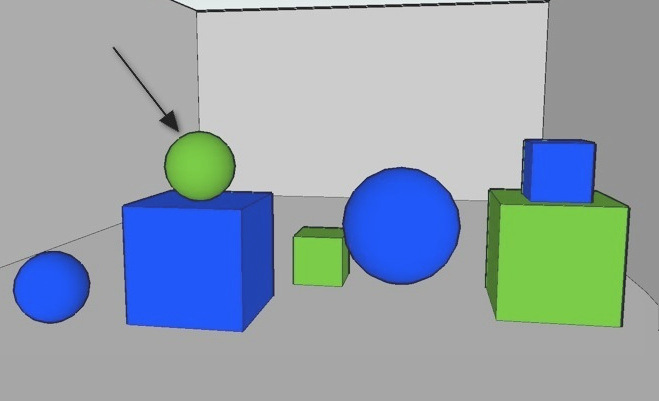
\includegraphics[width=\textwidth]{images/3.jpg}
%\vspace*{-.25cm}
%\vspace*{-.4cm}\caption{Input scene}
%\label{GRE3D7-stimulus}
%\end{minipage}
%\hspace*{-0.2cm}
%\begin{minipage}[b]{0.6\linewidth}
%\centering
%\begin{tikzpicture}
%  [
%    n/.style={circle,fill,draw,inner sep=3pt,node distance=1.4cm},
%    aArrow/.style={->, >=stealth, semithick, shorten <= 2pt, shorten >= 2pt},
%  ]
% \node[n,label=above:$e_1$,label=below:{
%    \relsize{-1}$\begin{array}{c}
%      \nLeft\\[-2pt]
%      \nSmall\\[-2pt] 
%      \nBlue \ \  
%      \nBall\end{array}$}] (a) {};

% \node[n,label=above:$e_2$,label=below:{
%    \relsize{-1}$\begin{array}{c}
%      \nLeft\\[-2pt]
%      \nBig\\[-2pt] 
%      \nBlue \ \  
%      \nCube\end{array}$}, right of=a] (b) {};

% \node[n,label=below:$e_3$,label=above:{
%    \relsize{-1}$\begin{array}{c}
%      \nTop \ \       \nLeft \ \ 
%      \nSmall \ \       \nGreen \ \ 
%      \nBall\end{array}$}, above of=b] (c) {};

% \node[n,label=above:$e_4$,label=below:{
%    \relsize{-1}$\begin{array}{c}
%      \nSmall\\[-2pt] 
%      \nGreen\\[-2pt] 
%      \nCube\end{array}$}, right of=b] (d) {};

% \node[n,label=above:$e_5$,label=below:{
%    \relsize{-1}$\begin{array}{c}
%      \nBig\\[-2pt] 
%      \nBlue\\[-2pt] 
%      \nBall\end{array}$}, right of=d] (e) {};

% \node[n,label=above:$e_6$,label=below:{
%    \relsize{-1}$\begin{array}{c}
%      \nBig\\[-2pt] 
%      \nGreen\\[-2pt] 
%      \nCube\end{array}$}, right of=e] (f) {};

% \node[n,label=below:$e_7$,label=above:{
%    \relsize{-1}$\begin{array}{c}
%      \nTop \ \ 
%      \nSmall\ \ 
%      \nBlue \ \  
%      \nCube\end{array}$}, above of=f] (g) {};

% \draw [aArrow,bend right=90] (b) to node[auto,swap]{\relsize{-1}$\nBelow$} (c);
% \draw [aArrow,bend right=90] (c) to node[auto,swap]{\relsize{-1}$\nOntop$} (b);

% \draw [aArrow,bend right=30] (d) to node[auto,swap]{\relsize{-1}$\nLeftof$} (e);
% \draw [aArrow,bend right=30] (e) to node[auto,swap]{\relsize{-1}$\nRightof$} (d);

% \draw [aArrow,bend right=90] (f) to node[auto,swap]{\relsize{-1}$\nBelow$} (g);
% \draw [aArrow,bend right=90] (g) to node[auto,swap]{\relsize{-1}$\nOntop$} (f);

% \draw[dotted] (-.65,-1.2) rectangle (7.1,2.1);

% \end{tikzpicture}
%\vspace*{-.4cm}\caption{Scene as a relational model}
%\label{GRE3D7-stimulus-graph}
%\end{minipage}
%\end{figure}

%On termination, the algorithm computes what are called the $\mathcal{L}$-similarity classes of the input model $\gM$. Intuitively, if two elements in the model belong to the same $\mathcal{L}$-similarity class, then $\mathcal{L}$ is not expressive enough to tell them appart (i.e, no formula in $\mathcal{L}$ can distinguish them). 

%The algorithm we discuss uses formulas of the $\el$ description logic language~\cite{baad:desc03} to describe refinement classes\footnote{Notice, though, that the particular formal language used is independent of the main algorithm, and different add$_{\mathcal{L}}$(R,$\varphi$,\RE) functions can be used depending on the language involved.}. 
%For a detailed description of $\el$, we refer to~\cite{baad:desc03}.  
%The interpretation of the $\el$ formula $\psi \sqcap \exists$R.$\varphi$ is the set of all elements that satisfy $\psi$ and that are related by relation R to some element that satisfy $\varphi$. 
%For example, the interpretation of the formula \emph{ball} $\sqcap \exists$\emph{leftof}.\emph{cube} is the set of all balls that are on the left of some cube.  

Luego de terminar, el algoritmo calcula lo que se llaman las $\mathcal {L}$- clases de semejanza del modelo de entrada de~$\gM $. Intuitivamente, si dos elementos en el modelo pertenecen a la misma $\mathcal {L}$- clase similitud, entonces~$\mathcal {L}$ no es lo suficientemente expresiva para diferenciarlos (es decir, no hay una f\'ormula en~$\mathcal {L }$ que pueda distinguirlos).
%aca faltaba algoluego de logicas
El algoritmo que discutimos utiliza f\'ormulas de $\el$ lenguaje de descripci\'on de la l\'ogica~\cite{baad:desc03} para describir clases de refinamiento \footnote {Note, sin embargo, que el lenguaje formal utilizado en particular es independiente del algoritmo principal, y diferentes add$_{\mathcal {L}}$(R,$\varphi $, \RE) funciones se pueden utilizar en funci\'on del idioma en cuesti\'on.}.
%Para una descripci\'on detallada de $\el$, nos referimos a~\cite{baad:desc03}.
La interpretaci\'on de las $\el$ f\'ormula $\psi \sqcap \exists $R.$ \varphi$ es el conjunto de todos los elementos que satisfagan~$\psi$ y que est\'an relacionados por relaci\'on R con alg\'un elemento que satisface $\varphi $.
Por ejemplo, existe la interpretaci\'on de la f\'ormula \emph{bola}$\sqcap$ \emph{leftof}. \emph{cubo} es el conjunto de todas las bolas que est\'an a la izquierda de alg\'un cubo.


%%We are now ready to describe Algorithms~\ref{algo:bisim-l} and~\ref{algo:bisim-add-el-over}. 

%\begin{figure}[!t]
%\small
%\centering
%\begin{algorithm}[H]
%\dontprintsemicolon
%\caption{Computing $\mathcal{L}$-similarity classes}\label{algo:bisim-l}
%\KwIn{\footnotesize A model $\gM$ and a list Rs $\in (\REL \times [0,1])^*$
% of relation symbols with their \puse\ values, ordered by \puse}
%\KwOut{\footnotesize A set of formulas \RE such that
%$\{\interp{\varphi} \mid \varphi \in \RE\}$ is the set of
%$\mathcal{L}$-similarity classes of $\gM$}

%$\RE \leftarrow \{\top\}$\tcp*[f]{\footnotesize the most general description $\top$ applies to all elements in the scene}

%\For{\em (R,R.\puse) $\in$ Rs}{
%	R.\randomuse = Random(0,1)\tcp*[f]{\footnotesize R.\randomuse is the probability of using R} \;
%        R.\incuse = (1 $-$ R.\puse) / MaxIterations\tcp*[f]{\footnotesize R.\puse\ are incremented by R.\incuse in each loop}
%}

%\Repeat{\em $\forall$((R,R.\puse) $\in$ Rs).(R.\puse $\ge$ 1)\tcp*[f]{\footnotesize R.\puse\ are incremented until they reach 1}}{
%  \While(\tcp*[f]{\footnotesize while some class has at least two elements}){\em $\exists (\varphi \in$ \RE)$.(\#\interp{\varphi}>1)$}{
%      \RE' $\leftarrow$ \RE \tcp*[f]{\footnotesize make a copy for future comparison} \;
%      \For{\em (R, R.\puse) $\in$ Rs}{
%          \If(\tcp*[f]{\footnotesize R will be used in the expression}){\em R.\randomuse $\le$ R.\puse}{
%              \lFor{\em $\varphi \in$ \RE}{
%                  add$_\mathcal{EL}$(R, $\varphi$, \RE)\tcp*[f]{\footnotesize refine all classes using R}}
%                  }\;
%              \If(\tcp*[f]{\footnotesize the classification has changed}){\em \RE $\not =$ \RE'}{exit\tcp*[f]{\footnotesize exit for-loop to try again highest R.\puse}}
%              }
%     \If(\tcp*[f]{\footnotesize the classification has stabilized}){\em \RE $=$ \RE'}{exit\tcp*[f]{\footnotesize exit while-loop to increase R.\puse}}
%  }
%  \lFor{\em (R,R.\puse) $\in$ Rs}{
%    R.\puse $\leftarrow$ R.\puse $+$ R.\incuse\tcp*[f]{\footnotesize increase R.\puse}
%  }
%}
%\end{algorithm}

%\begin{algorithm}[H]
%\dontprintsemicolon
%\caption{add$_\el$(R, $\varphi$, \RE)} \label{algo:bisim-add-el-over}


%\begin{figure}[t]
%\small
%\centering
%\begin{algorithm}[H]
%\dontprintsemicolon
%\caption{add$_\el$(R, $\varphi$, \RE)} \label{algo:bisim-add-el-over}

%\If(\tcp*[f]{\footnotesize are we in the first loop?}){\em FirstLoop?}{
%    Informative $\leftarrow$ TRUE \tcp*[f]{\footnotesize allow overspecification}}
%\lElse(\tcp*[f]{\footnotesize informative:smaller than the original?}) {Informative $\leftarrow$ $\interp{\psi \sqcap \exists \mbox{\em R}.\varphi} \neq \interp{\psi}$} 
%\For{\em $\psi \in$ \RE with $\#\interp{\psi} > 1$}{
%  \If{\em $\psi \sqcap \exists$R.$\varphi$ is not subsumed in \RE\ {\bf and} \tcp*[f]{\footnotesize non-redundant:can't be obtained from \RE?}\\
%    \em \ \ \ $\interp{\psi \sqcap \exists \mbox{\em R}.\varphi} \neq \emptyset$ {\bf and} \tcp*[f]{\footnotesize non-trivial:has elements?}\\
%     \ \ \  \emph{Informative}}{
%    add $\psi \sqcap \exists \mbox{R}.\varphi$ to $\RE$ \tcp*[f]{\footnotesize add the new class to the classification} \;
%    remove subsumed formulas from $\RE$ \tcp*[f]{\footnotesize remove redundant classes}
%  }
%}
%\end{algorithm}
%\vspace*{-.5cm}\caption{Refinement algorithm with probabilities and overspecification for the \el-language}\label{fig:algo3}

%\end{figure}

%Algorithm~\ref{algo:bisim-l} takes as input a model and a list Rs of pairs (R,R.\puse) that links each relation R $\in \REL$, the set of all relation symbols in the model,  to some probability of use R.\puse. 
%I.e., if $\REL$ is the set of all relation symbols in the model then Rs $\in (\REL \times [0,1])^*$. We assume Rs to be ordered by R.\puse. 

%The set $\RE$ will contain the formal description of the refinement classes and it is initialized by the most general description $\top$.  
%For each R, we first compute R.\randomuse, a random number in [0,1].  If R.\randomuse $\le$ R.\puse\ then we will use R to refine the set of classes.  The value of R.\puse\ will be incremented by R.$\incuse$ in each main loop, to ensure that all relations are, at some point, considered by the algorithm.  This ensures that a referring expression will be found if it exists; but gives higher probability to expressions using relations with a high R.\puse. 

%While $\RE$ contains descriptions that can be refined (i.e., classes with at least two elements) we will call the refinement function add$_\mathcal{L}$(R,$\varphi$,$\RE$) successively with each relation in Rs. A change in one of the classes, can trigger changes in others. For that reason, if $\RE$ changes, we exit the \textbf{for} loop to start again with the relations of higher R.\puse. If after trying to refine the set with all relations in Rs, the set $\RE$ has not changed, then we have reached a stable state (i.e., the classes described in $\RE$ cannot be further refined with the current R.\puse\ values). We will then increment all the R.\puse\ values and start the procedure again. 

%Algorithm~\ref{fig:algo1} almost coincides with the one in~\cite{arec2:2008:Areces}.  The \textbf{for} loop will refine each descriptions in $\RE$ using the relation R and the other descriptions already in $\RE$, under certain conditions. The new description should be \emph{non-redundant} (it cannot be obtained from classes already in $\RE$), \emph{non-trivial} (it is not empty), and \emph{informative} (it does not coincide with the original class).  If these conditions are met, the new description is added to $\RE$, and redundant descriptions created by the new description are eliminated. The \textbf{if} statement at the beginning of Algorithm in Figure~\ref{fig:algo2} disregards the informativity test during the first loop of the algorithm allowing overspecification.    

%Suppose fixed an input model $\gM$ and values for Rs, and fix also some target element $t$.  Assume also that $t$ indeed has an $\el$-referring expression.  Upon termination, Algorithm~\ref{fig:algo1} will compute an $\el$ formula $\varphi$ such that $\interp{\varphi} = \{t\}$, but $\varphi$ might be different in each run of the algorithm (even though $\gM$ and Rs are fixed).  If we repeat this experiment a statistically significant number of times, we can define an estimate of the probability distribution of the REs generated by the algorithm for $t$, given $\gM$ and Rs. In Section~\ref{sec:evaluation} we will show that given a corpus of REs for $\gM$, it is possible to define R.\puse\ values so that this probability distribution matches with good accuracy the probability distribution of REs found in the corpus.  


Algoritmo~\ref{algo:bisim-l} toma como entrada un modelo y una lista de pares (R, R \puse) Que une cada relaci\'on R$\in \REL $, el conjunto de todos los s\'{i}mbolos de relaci\'on en el modelo, en cierta probabilidad de uso R.\puse.
Es decir, si $\REL$ es el conjunto de todos los s\'{i}mbolos de relaci\'on en el modelo a continuaci\'on, R$\in (\REL \ \times [0,1]) ^ * $. Suponemos Rs estan ordenados de mayor a menor por R.\puse.

El conjunto $\RE$ contendr\'a la descripci\'on formal de las clases de refinamiento y es inicializado por la clase m\'as general $\top$. 
%Descripci\'on$\mayor de $.
Para cada R, primero calculamos R.\randomuse, un n\'umero aleatorio en [0,1]. Si R.\randomuse$\le$ R.\puse\ entonces vamos a utilizar R para refinar el conjunto de clases. El valor de R.\puse \ se incrementar\'a en R.$\incuse$ en cada bucle principal, para asegurar que todas las relaciones son, en alg\'un momento, consideradas por el algoritmo. Esto asegura que una expresi\'on referencial se encontrar\'a si existe; pero da mayor probabilidad a las expresiones que utilizan las relaciones con un alto R.\puse.

Mientras que $\RE$ contiene descripciones que pueden ser refinadas (es decir, las clases con al menos dos elementos) vamos a llamar a la funci\'on refinamiento add$_\mathcal {L}$(R,$\varphi $,$\RE$) sucesivamente con cada relaci\'on en Rs. Un cambio en una de las clases, puede desencadenar cambios en las dem\'as. Por esa raz\'on, si $\RE$ cambia, salimos del \textbf {for} bucle para empezar de nuevo con las relaciones de m\'as alto R.\puse. Si despu\'es de tratar de refinar el conjunto con todas las relaciones en R, el conjunto $\RE$ no ha cambiado, entonces hemos llegado a un estado estable (es decir, las clases descriptas en $\RE$ no pueden ser refinadas con los valores actuales de R.\puse). A continuaci\'on, se incrementar\'a todos los valores de R.\puse y se iniciar\'a el procedimiento de nuevo.

Algoritmo~\ref{fig:algo1} casi coincide con el de~\cite{arec2:2008:Areces}. El \ textbf {for} bucle refinar\'a cada descripciones en $\RE$ utilizando la relaci\'on R y las otras descripciones que ya est\'an en $\RE $, bajo ciertas condiciones. La nueva descripci\'on debe ser \emph{no redundante} (que no se puede obtener a partir de clases que ya est\'an en $\RE$ ), \emph{no trivial} (no ser vac\'{i}a), y \emph{informativa} (no debe coincidir con la clase original). Si se cumplen estas condiciones, la nueva descripci\'on se a\~nade a $\RE $, y las descripciones redundantes creadas por la nueva descripci\'on se eliminan. La declaraci\'on \textbf{if} al principio del algoritmo en la Figura~\ref{fig:algo2} no tiene en cuenta la prueba de informatividad durante el primer bucle del algoritmo que permite sobreespecificaci\'on.

Supongamos que fija un modelo de entrada de $\gM$ y los valores de R, y alg\'un elemento target $t$. Supongamos tambi\'en que $t$ efectivamente tiene una expresi\'on referencial en $\el$. Cuando termina, el Algoritmo~\ref{fig:algo1} d\'a $\el$ f\'ormulas $\varphi$ tal que $\interp{\varphi} = \{t\}$, pero $\varphi$ podr\'{i}a ser diferente en cada ejecuci\'on del algoritmo (a pesar de que $\gM$ y Rs son fijos). Si repetimos este experimento un n\'umero estad\'{i}sticamente significativo de veces, podemos definir una estimaci\'on de la distribuci\'on de probabilidad de las ER generadas por el algoritmo de $t $, dado $\gM$ y Rs. En la Secci\'on~\ref{sec:evaluacion} vamos a demostrar que dado un corpus para $\gM$, es posible definir R.\puse valores para que esta distribuci\'on de probabilidad coincida con buena precisi\'on la distribuci\'on de probabilidad encontrada en el corpus.


%\section{Aprendizaje autom\E1tico}

%\section{Agregando sobreespecificaci\F3n}
